\chapter{Quantum Many-Body Physics} \label{chp:quantum}
\epigraph{If you are not completely confused by quantum mechanics, you do not understand it.}{John Wheeler}
\begin{figure}[H]
	\centering
	\captionsetup[subfigure]{labelformat=empty}
	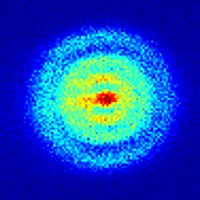
\includegraphics[scale=3.0]{Images/art_quantum.jpg}
	\caption{The first photograph of a Hydrogen atom was captured by an ultra sensitive camera in 2013. One can actually see the probability distribution $|\Psi(\bs{r})|^2$ with the naked eye. Published in Phys. rev. lett. 110, 213001 (2013), \textit{Hydrogen atoms under magnification}. \cite{stodolna_hydrogen_2013}}
\end{figure}
Around 1900, some physicists thought that there were nothing new to be discovered in physics and all that remained was more precise measurements, as Lord Kelvin famously pointed out. \cite{weisstein_kelvin_2007} He could not have been more wrong. In the following years, things were observed that could only be described by a quantized theory, led by Albert Einstein's explanation of the photoelectric effect in 1905. 

Immense efforts were placed on completing the theory, and contributions from an array of scientists over a period of 20 years were necessary to get it finished. In 1929, Paul Dirac stated something similar to what Lord Kelvin said 30 years earlier, but apparently with greater accuracy. 

\newpage
\section{Introductory Quantum Physics} \label{subsec:elementary}
In this section we will present the fundamentals of the quantum theory, that will make up the framework of this project. The theory is based on David Griffith's incredible textbook, \textit{Introduction to Quantum Mechanics}, where the reader is relegated for in-depth information.

Before we get started, we make a few assumptions in order to simplify our problem. They most important ones are specified below with an explanation why they are valid.

\begin{itemize}
	\item \textbf{Point-like particles:} First, all particles involved will be assumed to be point-like, i.e, that they lack spatial extension. This includes the nucleus in atomic systems, but it still makes sense since the distance from the nucleus to the electrons is known to be much larger then the nucleus extent.
	
	\item \textbf{Non-relativistic spacetime:}  Second, we operate in the non-relativistic spacetime, which is valid as long as we do not approach the speed of light and we do not involve strong forces. Applying classical physics, we can find that the speed of the electron in a hydrogen atom is about 1\% of the speed of light, and even though the electrons get higher speed in heavier atoms, we do not need to worry about it. The forces acting are the weak Coulomb forces.
	
	\item For specific systems we might make new assumptions and approximations. For instance, for atomic systems we will assume that the nucleus is at rest. Those approximations will be discussed consecutively. 
\end{itemize}

\subsection{The Schrödinger Equation} \label{subsec:schrodinger}
The Schrödinger equation is a natural starting point, which gives the energy eigen states of a system defined by a Hamiltonian $\hat{\mathcal{H}}$ and its eigen functions, $\Psi$, which are the wave functions. The time-independent Schrödinger equation reads
\begin{equation}
\label{eq:Energy}
 \hat{\mathcal{H}}\psin=\epsilon_n\psin
\end{equation}
where the Hamiltonian is the total energy operator. By analogy with the classical mechanics, this is given by
\begin{equation}
\hat{\mathcal{H}}=\hat{\mathcal{T}}+\hat{\mathcal{V}}
\end{equation}
with $\hat{\mathcal{T}}$ and $\hat{\mathcal{V}}$ as the kinetic and potential energy operators respectively. 

The kinetic energy yields $T=p^2/2m$, such that the kinetic energy operator can be represented as 
\begin{equation}
\hat{\mathcal{T}}=\frac{\hat{\mathcal{P}}^2}{2m}
\end{equation}
according to Ehrenfest's theorem. Further, the momentum operator is $\hat{\mathcal{P}}=-i\hbar\nabla$.

The potential energy can be split into an external part and an interaction part, where the latter is given by the Coulomb interaction. For two identical particles of charge $q$, the repulsive interaction gives the energy
\begin{equation}
V_I=k\frac{q^2}{r_{12}}
\end{equation}
where $r_{12}$ is the distance between the particles. The total Hamiltonian of a system of $P$ identical particles takes the form
\begin{equation}
\hat{\mathcal{H}}=-\sum_i^P\frac{\hbar^2}{2m}\nabla_i^2+\sum_i^{}u_i + \sum_i^P\sum_{j>i}^Pk\frac{q^2}{r_{ij}}
\label{eq:ElectronicHamiltonian}
\end{equation}
which is the farthest we can go without specifying the external potential $u_i$. $r_{ij}$ is the relative distance between particle $i$ and $j$, defined by $r_{ij}\equiv|\bs{r}_i-\bs{r}_j|$.

Setting up equation \eqref{eq:Energy} with respect to the energies, we obtain an integral,
\begin{equation}
\epsilon_n=\frac{\int d\bs{r}\psinc\hatH\psin}{\int d\bs{r}\psinc\psin},
\label{eq:energyintegral}
\end{equation}
which not necessarily is trivial to solve. If we take the wave function squared we get the probability distribution,
\begin{equation}
P(\bs{r})=\psinc\psin=|\psin|^2
\end{equation}
so the nominator is simply the integral over all probabilities. If the wave function is normalized correctly, this should always give 1. Assuming that is the case, the expectation value can be expressed more elegantly by using Dirac notation,
\begin{equation}
E[\Psi]=\mel{\Psi}{\hatH}{\Psi},
\end{equation}
where the first part, $\bra{\Psi}$ is called a bra and the last part, $\ket{\Psi}$ is called a ket. At first this might look artificial and less informative, but it simplifies the notation significantly. More information about the notation is found in Appendix A. 

In many cases we do not know the exact wave function, and need to rely on a trial wave function guess. Henceforth, we will use $\Psi$ as the exact total wave function, $\psi$ as the exact single particle function (SPF), $\Psi_T$ as the total trial wave function and $\phi$ as the trial SPF. 
\cite{griffiths_introduction_2005}

\subsection{The Variational Principle}
In the equations above, the presented wave functions are assumed to be the exact eigen functions of the Hamiltonian. But often we do not know the exact wave functions, and we need to guess what the wave functions might be. In those cases we make use of the variational principle, which states that only the exact ground state wave function is able to give the ground state energy. All other wave functions that fulfill the required properties (see section \ref{subsec:wavefunction}) give higher energies, and mathematically we can express the statement
\begin{equation}
\epsilon_0\leq\mel{\Psi_T}{\hat{\mathcal{H}}}{\Psi_T}.
\label{eq:variationalprinciple}
\end{equation}

Variational Monte-Carlo is a method based on (and named after) the variational principle, where we vary the trial wave function in order to obtain the lowest energy. It will be detailed in chaper \eqref{chp:methods}.

\subsection{Postulates of Quantum Mechanics}
The quantum theory is built on a few fundamental postulates, which will always be true. Before we go further, we will take a quick look at some of them.

\begin{enumerate}
\item Associated with any particle moving in a conservative field of force is a wave function which determines everything that can be known about the system.

\item With every physical observable q there is associated an operator Q, which when operating upon the wave function associated with a definite value of that observable will yield that value times the wave function.

\item Any operator Q associated with a physically measurable property q will be Hermitian.

\item The set of eigen functions of operator Q will form a complete set of linearly independent functions.

\item For a system described by a given wave function, the expectation value of any property q can be found by performing the expectation value integral with respect to that wave function.

\item The time evolution of the wave function is given by the time-dependent Schrodinger equation. 
\end{enumerate}

\section{The Trial Wave Function} \label{subsec:wavefunction}
By the first postulate of quantum mechanics, the wave function contains all the information specifying the state of the system. This means that all observable in classical mechanics can also be measured from the wave function, which makes finding the wave function our main goal.

The trial wave function needs to meet some requirements in order to be used in the variational principle, and we thus need to make an educated guess on the wave function where the requirements are fulfilled. The requirements are the following:

\begin{enumerate}
	\item \textbf{Normalizability:} The wave function needs to be normalizable to make physical sense. The total probability should always be 1, and a wave function that cannot be normalized will not have a finite total probability. The consequence is that the wave function needs to converge to zero when the positions get large. 
	
	\item \textbf{Cusp condition:} The cusp condition (also called the Kato theorem) states that the wave function should have a cusp where the potential explodes. An example on this is when charged particles come close to each other. 
	
	\item \textbf{Symmetry and anti-symmetry:} The wave function needs to be either symmetric or anti-symmetric under exchange of two coordinates, dependent on whether the particles are fermions or bosons. More about this in the next section.
\end{enumerate}

\subsection{Bosons and fermions} \label{subsubsec:symmetry}
Assume that we have a permutation operator $\hat{P}$ which exchanges two coordinates in the wave function,
\begin{equation}
\hat{P}(i\rightarrow j)\Psi_n(\bs{x}_1,\hdots,\bs{x}_i,\hdots,\bs{x}_j,\hdots,\bs{x}_M)=p\Psi_n(\bs{x}_1,\hdots,\bs{x}_j,\hdots,\bs{x}_i,\hdots,\bs{x}_M),
\end{equation}
where $p$ is just a factor which comes from the transformation. If we again apply the $\hat{P}$ operator, we should switch the same coordinates back, and we expect to end up with the initial wave function. For that reason, $p=\pm1$. \footnote{Actually, in two-dimensional systems we have a third possibility which gives an \textit{anyon}. The theory on this was developed by J.M. Leinaas and J. Myrheim during the 1970's. \cite{leinaas_one_1977}}

The particles that have an antisymmetric (AS) wavefunction under exchange of two coordinates are called fermions, named after Enrico Fermi, and have half integer spin. On the other hand, the particles that have a symmetric (S) wavefunction under exchange of two coordinates are called bosons, named after Satyendra Nath Bose, and have integer spin. 

It turns out that because of their antisymmetric wavefunction, two identical fermions cannot be found at the same position at the same time, known as the Pauli principle. This causes some difficulties when dealing with multiple fermions, because we always need to ensure that the total wavefunction becomes zero if two identical particles happen to be at the same position. To do this, we introduce a Slater determinant as described below. In this particular project, we are going to focus on electrons and therefore fermions. However, much of the theory applies for bosons as well.

\subsection{Slater determinant} \label{subsec:slater}
For a system of more particles we can define a total wavefunction, which is a composition of all the single particle wavefunctions (SPF) and contains all the information about the system. For fermions we need to compile the SPFs such that the Pauli principle is fulfilled at all times. One way to do this is by setting up the SPFs in a determinant, known as a Slater determinant.

Consider a system of two identical fermions with SPFs $\phi_1$ and $\phi_2$ at positions $\boldsymbol{r}_1$ and $\boldsymbol{r}_2$ respectively. The way we define the wavefunction of the system is then
\begin{equation}
\Psi_T(\bs{r}_1,\bs{r}_2)=
\begin{vmatrix}
\phi_1(\boldsymbol{r}_1) & \phi_2(\boldsymbol{r}_1)\\
\phi_1(\boldsymbol{r}_2) & \phi_2(\boldsymbol{r}_2)
\end{vmatrix}
=\phi_1(\boldsymbol{r}_1)\phi_2(\boldsymbol{r}_2)-\phi_2(\boldsymbol{r}_1)\phi_1(\boldsymbol{r}_2),
\end{equation}
which is set to zero if the particles are at the same position. The determinant yields the same no matter how big the system is.

The Slater determinant is just an ansatz since it does not come from any analytical calculations, and we therefore need to denote it as the trial wave function. Additionally, the Slater determinant above contains the radial part only, because the single particle functions are the radial part by convention. For a general Slater determinant, the spin part needs to be included as well, giving 
\begin{equation}
\Psi(\boldsymbol{r}_1,\boldsymbol{r}_2,\hdots,\boldsymbol{r}_N)=
\begin{vmatrix}
\psi_1(\boldsymbol{r}_1) & \psi_2(\boldsymbol{r}_1) & \hdots & \psi_N(\boldsymbol{r}_1)\\
\psi_1(\boldsymbol{r}_2) & \psi_2(\boldsymbol{r}_2) & \hdots & \psi_N(\boldsymbol{r}_2)\\
\vdots & \vdots & \ddots & \vdots & \vdots\\
\psi_1(\boldsymbol{r}_N) & \psi_2(\boldsymbol{r}_N) & \hdots & \psi_N(\boldsymbol{r}_N)
\end{vmatrix}
\end{equation}
where the $\psi$'s are the true single particle wave functions, which are the tensor products 
\begin{equation}
\psi=\phi\otimes\xi
\end{equation}
with $\xi$ as the spin part. How the spin can be factorized out for electronic systems will be shown below. 

Similar to the Slater determinant, a Slater permanent might be included for bosonic systems. The permanent of a matrix is similar to the determinant, but all negative signs are replaced by positive signs. 

\subsection{Simplification of Slater determinant for electronic systems} \label{subsubsec:electronsystem}
For our purpose we will study fermions of spin $\sigma=\pm 1/2$ only, i.e., electrons and protons. In this particular case, the SPFs can be arranged in spin-up and spin-down parts, such that the Slater determinant can be simplied to 
\begin{equation*}
\Psi(\boldsymbol{r}_1,\boldsymbol{r}_2,\hdots,\boldsymbol{r}_N)=
\begin{vmatrix}
\phi_1(\boldsymbol{r}_1)\xi_{\uparrow} & \phi_1(\boldsymbol{r}_1)\xi_{\downarrow} & \hdots & \phi_{N/2}(\boldsymbol{r}_1)\xi_{\uparrow} & \phi_{N/2}(\boldsymbol{r}_1)\xi_{\downarrow}\\
\phi_1(\boldsymbol{r}_2)\xi_{\uparrow} & \phi_1(\boldsymbol{r}_2)\xi_{\downarrow} & \hdots & \phi_{N/2}(\boldsymbol{r}_2)\xi_{\uparrow} & \phi_{N/2}(\boldsymbol{r}_2)\xi_{\downarrow}\\
\vdots & \vdots & \ddots & \vdots & \vdots\\
\phi_1(\boldsymbol{r}_{N-1})\xi_{\uparrow} & \phi_1(\boldsymbol{r}_{N-1})\xi_{\downarrow} & \hdots & \phi_{N/2}(\boldsymbol{r}_{N-1})\xi_{\uparrow} & \phi_{N/2}(\boldsymbol{r}_{N-1})\xi_{\downarrow}\\
\phi_1(\boldsymbol{r}_N)\xi_{\uparrow} & \phi_1(\boldsymbol{r}_N)\xi_{\downarrow} & \hdots & \phi_{N/2}(\boldsymbol{r}_N)\xi_{\uparrow} & \phi_{N/2}(\boldsymbol{r}_N)\xi_{\downarrow}
\end{vmatrix}.
\end{equation*}
Here we assume that two particles of opposite spin are found at the same position, which makes the number of fermions with spin up equal to the number of fermions with spin down. This is obviously not a assumption that always will hold, but it eases the calculations. 

Now recall that all particles with odd position indices ($\bs{r}_1$, $\bs{r}_3$, $\hdots$) have spin up, such that $\phi_j(\bs{r}_i)\xi_{\downarrow}=0$ where $j=1,\hdots,N/2$ and $i$ spans over all the odd positions indices. The same applies for particles with even position indices and spin down, and we get 
\begin{equation*}
\Psi(\boldsymbol{r}_1,\boldsymbol{r}_2,\hdots,\boldsymbol{r}_N)=
\begin{vmatrix}
\phi_1(\boldsymbol{r}_1)\xi_{\uparrow} & 0 & \hdots & \phi_{N/2}(\boldsymbol{r}_1)\xi_{\uparrow} & 0\\
0 & \phi_1(\boldsymbol{r}_2)\xi_{\downarrow} & \hdots & 0 & \phi_{N/2}(\boldsymbol{r}_2)\xi_{\downarrow}\\
\vdots & \vdots & \ddots & \vdots & \vdots\\
\phi_1(\boldsymbol{r}_{N-1})\xi_{\uparrow} & 0 & \hdots & \phi_{N/2}(\boldsymbol{r}_{N-1})\xi_{\uparrow} & 0\\
0 & \phi_1(\boldsymbol{r}_N)\xi_{\downarrow} & \hdots & 0 & \phi_{N/2}(\boldsymbol{r}_N)\xi_{\downarrow}
\end{vmatrix},
\end{equation*}
which by row operations can be found to be row equivalent with
\begin{equation*}
\Psi(\boldsymbol{r}_1,\boldsymbol{r}_2,\hdots,\boldsymbol{r}_N)=
\begin{vmatrix}
\phi_1(\boldsymbol{r}_1)\xi_{\uparrow} & \phi_2(\boldsymbol{r}_1)\xi_{\uparrow} & \hdots & 0 & 0\\
\phi_1(\boldsymbol{r}_3)\xi_{\uparrow} & \phi_2(\boldsymbol{r}_3)\xi_{\uparrow} & \hdots & 0 & 0\\
\vdots & \vdots & \ddots & \vdots & \vdots\\
0 & 0 & \hdots & \phi_{N/2-1}(\boldsymbol{r}_{N-2})\xi_{\downarrow} & \phi_{N/2}(\boldsymbol{r}_{N-2})\xi_{\downarrow}\\
0 & 0 & \hdots & \phi_{N/2-1}(\boldsymbol{r}_N)\xi_{\downarrow} & \phi_{N/2}(\boldsymbol{r}_N)\xi_{\downarrow}
\end{vmatrix}.
\end{equation*}
This means that we can split the Slater determinant in a spin up part and a spin down part,
\begin{equation}
\Psi(\boldsymbol{r}_1,\boldsymbol{r}_2,\hdots,\boldsymbol{r}_N)=|\hat{D}_{\uparrow}|\cdot |\hat{D}_{\downarrow}|
\end{equation}
which saves us from a lot of computations. For a detailed explanation of the splitting, appendix I of Daniel Nissenbaum's dissertation is an excellent read. \cite{nissenbaum_stochastic_2008} Szabo \& Ostlund in \cite{szabo_modern_1996} is also a good explanation. 

\subsection{Basis set} \label{subsec:basisset}
To go further, we need to define a basis set, $\phi_n(\bs{r})$ which should be chosen carefully based on the system. For a few systems, we know the exact basis of the non-interacting case, and it is thus a natural basis to use in the Slater determinant. For other systems, the choice of basis might depend on the situation, where we typically need to weigh computational time against accuracy. Concrete examples on both cases will be presented in chapter \eqref{chp:systems}.

Often, one will see that the basis is optimized by the Hartree-Fock method. Using this basis in a single Slater determinant, we obtain the Hartree-Fock energy which sometimes is quite accurate. To get an even better energy estimate, we need to add more Slater determinants, which is the task of the post Hartree-Fock methods. More about this in chapter (\ref{chp:methods}-\ref{chp:posthartreefock}).

\subsection{Jastrow factor} \label{subsubsec:jastrow}
From electrostatics we know that identical, charged particles will repel each other. This means that the probability of finding two particles close to each other should be low, which needs to be baked into the wave function. One way to do this is to simply multiply the wave function with the distance between the particles; the smaller distance the lower probability. Nevertheless, this does not fulfill the normalizability requirement of the trial wave function, but the same idea lies behind the Padé-Jastrow factor, which reads
\begin{equation}
J(\bs{r}; \beta, \gamma) = \exp\bigg(\sum_{i=1}^P\sum_{j>i}^P\frac{a_{ij}r_{ij}}{1+\beta r_{ij}}\bigg).
\label{eq:PadeJastrow}
\end{equation}
where $r_{ij}$ again is the relative distance between particle $i$ and $j$, $\beta$ is a variational parameter, while $a_{ij}$ depends on the spin of the interacting objects in the following way:
\begin{equation}
\label{eq:ajastrow}
a_{ij}=
\begin{cases} 
e^2/(d+1) & \text{if $i,j$ are particles of same spin} \\
e^2/(d-1) & \text{if $i,j$ are particles of opposite spin},
\end{cases}
\end{equation}
for dimensions $d\in[2,3]$ where $e$ is the elementary charge. We will later use natural and atomic units, and set $e=1$, which for two dimensions gives $a_{ij}=1/3$ (same spin) or $a_{ij}=1$ (opposite spin) and for three dimensions $a_{ij}=1/4$ (same spin) and $a_{ij}=1/2$ (opposite spin).

This Jastrow factor is known to give accurate results for fermions and bosons because it gives the correct cusp condition, and it is the one we gonna use in the standard variational Monte-Carlo simulations.





